\documentclass[answers]{exam}
\usepackage[english]{babel}
\usepackage[utf8x]{inputenc}
\usepackage{amsmath,amssymb,amsthm,mathtools}

\title{OPER 510 - Introduction to Mathematical Programming%
	\\ Midterm}
\author{Brandon Hosley}
\date{\today}

\usepackage[table,dvipsnames]{xcolor}
\usepackage{graphicx}
\usepackage{nicefrac}
\usepackage{enumitem}
\usepackage{multicol}
\usepackage{setspace}
\usepackage[final]{pdfpages}

\begin{document}
\includepdf[pages=-]{Midterm Agreement Signed.pdf}
\maketitle
\unframedsolutions

\begin{questions}
	
%%%%%%%%%%%%%%%%%%%%%%%%%%%
% 	\begin{ Question 1}	  %
%%%%%%%%%%%%%%%%%%%%%%%%%%%
\question
\begin{parts}
	\part Via the simplex method, find the solution to the following problem:
	\begin{flalign*}
		\text{Max } z=90x_1 +40x_2 +10x_3 +30x_4            &         &  \\
		\text{s.t.}\hspace{2.5em} 15x_1 +10x_2 +10x_3 + \,\ 5x_4 & \leq 45 &  \\
		15x_1+ \,\ 5x_2+ \,\ 5x_3+ \,\ 5x_4                             & \leq 35 &  \\
		x_1 \hspace{22.5ex}                                    & \geq 1  &  \\
		x_3 \hspace{7ex}                                    & \geq 2  &  \\
		x_1,x_2,x_3,x_4                                     & \geq 0  &
	\end{flalign*}

	\part The General Service Organization, GSO, has contracted to sell certain quantities of a particular product over the next four months. Because of variations in the size of the labor force, the production capacity and materials, costs vary from month to month. Storage costs are incurred on any items carried over to the next month, but not on items sold in the same month that they are produced. The costs and requirements are summarized below: \bigskip \\
	\begin{tabular}{ccccc}
		& Contracted & Production & Production & Storage \\
		\underline{Month} & \underline{Sales} & \underline{Capacity} & \underline{Cost/Unit (\$)} & \underline{Cost/Unit/Month (\$)} \\
		1 & 60 & 90 & 70 & 2 \\
		2 & 70 & 60 & 72 & 1 \\
		3 & 90 & 80 & 70 & 1 \\
		4 & 70 & 100 & 65 & 3 \\
	\end{tabular} \bigskip \\
	Initial inventory is 20 units. For service reasons, GSO wants to maintain at least 5 units of inventory at the end of each month. \textit{Formulate} a linear programming model to determine GSO’s production and inventory schedule.
	
	\part Give the rank of the following system of equations: 
	\begin{flalign*}
		2x_1 +\ \ 3x_2 +4x_3 &=3 &\\
		4x_1 +\ \ 5x_2 +1x_3 &=2 &\\
		 x_1 +1.5x_2 +2x_3 &=3/2 &\\
	\end{flalign*}
	
	\part Solve the following linear program.
	\begin{flalign*}
		\text{Max } z=10x_1 +3x_2 +12x_3 & & \\
		\text{s.t.}\hspace{3em} 2x_1 +1x_2+ \,\ 5x_3 &\leq 20 & \\
		x_1, x_2, x_3 &\geq 0 & \\
	\end{flalign*}
\end{parts}

\begin{solution}
\begin{parts}
	\part % Q1-A
	\noindent 
	\def \ProbOneScale {0.8}
	
	\scalebox{\ProbOneScale}{
	\begin{tabular}{cccccccccccccc}
		$c_j$                   &                            &                                & 90    & 40    & 10    & 30    & 0     & 0     & 0     & 0     & -M    & -M    &           \\
		\multicolumn{1}{c|}{}   & \multicolumn{1}{c|}{bv}    & \multicolumn{1}{c|}{RHS}       & $x_1$ & $x_2$ & $x_3$ & $x_4$ & $s_1$ & $s_2$ & $s_3$ & $s_4$ & $A_1$ & $A_2$ & ratio     \\ \cline{1-13}
		\multicolumn{1}{c|}{0}  & \multicolumn{1}{c|}{$s_1$} & \multicolumn{1}{c|}{45}        & 15    & 10    & 10    & 5     & 1     & 0     & 0     & 0     & 0     & 0     & 45/15=3   \\
		\multicolumn{1}{c|}{0}  & \multicolumn{1}{c|}{$s_2$} & \multicolumn{1}{c|}{35}        & 15    & 5     & 5     & 5     & 0     & 1     & 0     & 0     & 0     & 0     & 35/15=2.3 \\
		\multicolumn{1}{c|}{-M} & \multicolumn{1}{c|}{$A_1$} & \multicolumn{1}{c|}{1}         & 1     & 0     & 0     & 0     & 0     & 0     & -1    & 0     & 1     & 0     & 1/1=1     \\
		\multicolumn{1}{c|}{-M} & \multicolumn{1}{c|}{$A_2$} & \multicolumn{1}{c|}{2}         & 0     & 0     & 1     & 0     & 0     & 0     & 0     & -1    & 0     & 1     & 0         \\ \cline{1-13}
		& \multicolumn{1}{c|}{$z_j$} & \multicolumn{1}{c|}{-2M}       & -M    & 0     & -M    & 0     & 0     & 0     & M     & M     & -M    & -M    &           \\ \cline{3-13}
		&                            & \multicolumn{1}{c|}{$c_j-z_j$} & 90+M  & 0     & 10+M  & 0     & 0     & 0     & -M    & -M    & 0     & 0     &          
	\end{tabular} } % End scalebox

	Enter on $x_1$, exit $A_1$ \\
	R1 - 15R3 \\
	R2 - 15R3
	
	\scalebox{\ProbOneScale}{ 
	\begin{tabular}{cccccccccccccc}
		$c_j$                   &                            &                                & 90    & 40    & 10    & 30    & 0     & 0     & 0     & 0     & -M    & -M    &         \\
		\multicolumn{1}{c|}{}   & \multicolumn{1}{c|}{bv}    & \multicolumn{1}{c|}{RHS}       & $x_1$ & $x_2$ & $x_3$ & $x_4$ & $s_1$ & $s_2$ & $s_3$ & $s_4$ & $A_1$ & $A_2$ & ratio   \\ \cline{1-13}
		\multicolumn{1}{c|}{0}  & \multicolumn{1}{c|}{$s_1$} & \multicolumn{1}{c|}{30}        & 0     & 10    & 10    & 5     & 1     & 0     & 15    & 0     & 0     & 0     & 30/10=3 \\
		\multicolumn{1}{c|}{0}  & \multicolumn{1}{c|}{$s_2$} & \multicolumn{1}{c|}{20}        & 0     & 5     & 5     & 5     & 0     & 1     & 15    & 0     & 0     & 0     & 20/5=4  \\
		\multicolumn{1}{c|}{90} & \multicolumn{1}{c|}{$x_1$} & \multicolumn{1}{c|}{1}         & 1     & 0     & 0     & 0     & 0     & 0     & -1    & 0     & 1     & 0     & 0       \\
		\multicolumn{1}{c|}{-M} & \multicolumn{1}{c|}{$A_2$} & \multicolumn{1}{c|}{2}         & 0     & 0     & 1     & 0     & 0     & 0     & 0     & -1    & 0     & 1     & 2/1=2   \\ \cline{1-13}
		& \multicolumn{1}{c|}{$z_j$} & \multicolumn{1}{c|}{90-2M}     & 90    & 0     & -M    & 0     & 0     & 0     & -90   & M     & 90    & -M    &         \\ \cline{3-13}
		&                            & \multicolumn{1}{c|}{$c_j-z_j$} & 0     & 40    & 10+M  & 0     & 0     & 0     & 90    & -M    & -M-90 & 0     &        
	\end{tabular} } %end scalebox
	
	Enter $x_3$, exit $A_2$ \\
	R1 - 10R4 \\
	R2 - 5R4
	
	\scalebox{\ProbOneScale}{ 
	\begin{tabular}{cccccccccccccc}
		$c_j$                   &                            &                                & 90    & 40    & 10    & 30    & 0     & 0     & 0     & 0     & -M    & -M    &           \\
		\multicolumn{1}{c|}{}   & \multicolumn{1}{c|}{bv}    & \multicolumn{1}{c|}{RHS}       & $x_1$ & $x_2$ & $x_3$ & $x_4$ & $s_1$ & $s_2$ & $s_3$ & $s_4$ & $A_1$ & $A_2$ & ratio     \\ \cline{1-13}
		\multicolumn{1}{c|}{0}  & \multicolumn{1}{c|}{$s_1$} & \multicolumn{1}{c|}{10}        & 0     & 10    & 0     & 5     & 1     & 0     & 15    & 10    & -15   & -10   & 10/15=0.6 \\
		\multicolumn{1}{c|}{0}  & \multicolumn{1}{c|}{$s_2$} & \multicolumn{1}{c|}{10}        & 0     & 5     & 0     & 5     & 0     & 1     & 15    & 5     & 0     & -5    & 10/15=0.6 \\
		\multicolumn{1}{c|}{90} & \multicolumn{1}{c|}{$x_1$} & \multicolumn{1}{c|}{1}         & 1     & 0     & 0     & 0     & 0     & 0     & -1    & 0     & 1     & 0     & 1/-1=-1   \\
		\multicolumn{1}{c|}{10} & \multicolumn{1}{c|}{$x_3$} & \multicolumn{1}{c|}{2}         & 0     & 0     & 1     & 0     & 0     & 0     & 0     & -1    & 0     & 1     & 0         \\ \cline{1-13}
		& \multicolumn{1}{c|}{$z_j$} & \multicolumn{1}{c|}{110}       & 90    & 0     & 10    & 0     & 0     & 0     & -90   & -10   & 90    & 10    &           \\ \cline{3-13}
		&                            & \multicolumn{1}{c|}{$c_j-z_j$} & 0     & 40    & 0     & 30    & 0     & 0     & 90    & 10    & -M-90 & -M-10 &          
	\end{tabular} } %end scalebox

	Enter $s_3$, exit $s_2$ \\
	R2 / 15 \\
	R1 - 15R2 \\
	R3 + R2
	
	\scalebox{\ProbOneScale}{ 
	\begin{tabular}{cccccccccccccc}
		$c_j$                   &                            &                                & 90    & 40    & 10    & 30    & 0     & 0     & 0     & 0     & -M    & -M    &               \\
		\multicolumn{1}{c|}{}   & \multicolumn{1}{c|}{bv}    & \multicolumn{1}{c|}{RHS}       & $x_1$ & $x_2$ & $x_3$ & $x_4$ & $s_1$ & $s_2$ & $s_3$ & $s_4$ & $A_1$ & $A_2$ & ratio         \\ \cline{1-13}
		\multicolumn{1}{c|}{0}  & \multicolumn{1}{c|}{$s_1$} & \multicolumn{1}{c|}{0}         & 0     & 5     & 0     & 0     & 1     & -1    & 0     & 5     & -15   & -5    &               \\
		\multicolumn{1}{c|}{0}  & \multicolumn{1}{c|}{$s_3$} & \multicolumn{1}{c|}{2/3}       & 0     & 1/3   & 0     & 1/3   & 0     & 1/15  & 1     & 1/3   & 0     & -1/3  & (2/3)/(1/3)=2 \\
		\multicolumn{1}{c|}{90} & \multicolumn{1}{c|}{$x_1$} & \multicolumn{1}{c|}{5/3}       & 1     & 1/3   & 0     & 1/3   & 0     & 1/15  & 0     & 1/3   & 1     & -1/3  & (5/3)/(1/3)=5 \\
		\multicolumn{1}{c|}{10} & \multicolumn{1}{c|}{$x_3$} & \multicolumn{1}{c|}{2}         & 0     & 0     & 1     & 0     & 0     & 0     & 0     & -1    & 0     & 1     &               \\ \cline{1-13}
		& \multicolumn{1}{c|}{$z_j$} & \multicolumn{1}{c|}{170}       & 90    & 30    & 10    & 30    & 0     & 6     & 0     & 20    & 90    & -20   &               \\ \cline{3-13}
		&                            & \multicolumn{1}{c|}{$c_j-z_j$} & 0     & 10    & 0     & 0     & 0     & -6    & 0     & -20   & 90-M  & -20-M &              
	\end{tabular} } %end scalebox

	Enter $x_2$ exit $s_3$ \\
	R2 x 3 \\
	R1 - 5R2 \\
	R3 - 1/3R2
	
	\scalebox{\ProbOneScale}{
	\begin{tabular}{cccccccccccccc}
		$c_j$                   &                            &                                & 90    & 40    & 10    & 30    & 0     & 0     & 0     & 0     & -M    & -M    &       \\
		\multicolumn{1}{c|}{}   & \multicolumn{1}{c|}{bv}    & \multicolumn{1}{c|}{RHS}       & $x_1$ & $x_2$ & $x_3$ & $x_4$ & $s_1$ & $s_2$ & $s_3$ & $s_4$ & $A_1$ & $A_2$ & ratio \\ \cline{1-13}
		\multicolumn{1}{c|}{0}  & \multicolumn{1}{c|}{$s_1$} & \multicolumn{1}{c|}{-10}       & 0     & 0     & 0     & -5    & 1     & -2    & 0     & 0     & -15   & -10   &       \\
		\multicolumn{1}{c|}{40} & \multicolumn{1}{c|}{$x_2$} & \multicolumn{1}{c|}{2}         & 0     & 1     & 0     & 1     & 0     & 1/5   & 3     & 1     & 0     & -1    &       \\
		\multicolumn{1}{c|}{90} & \multicolumn{1}{c|}{$x_1$} & \multicolumn{1}{c|}{1}         & 1     & 0     & 0     & 0     & 0     & 0     & -1    & 0     & 1     & 0     &       \\
		\multicolumn{1}{c|}{10} & \multicolumn{1}{c|}{$x_3$} & \multicolumn{1}{c|}{2}         & 0     & 0     & 1     & 0     & 0     & 0     & 0     & -1    & 0     & 1     &       \\ \cline{1-13}
		& \multicolumn{1}{c|}{$z_j$} & \multicolumn{1}{c|}{190}       & 90    & 40    & 30    & 40    & 0     & 8     & 30    & 30    & 90    & -30   &       \\ \cline{3-13}
		&                            & \multicolumn{1}{c|}{$c_j-z_j$} & 0     & 0     & 0     & -10   & 0     & -8    & -30   & -30   & 90-M  & -30-M &      
	\end{tabular} } %end scalebox
	\bigskip \\

	\textbf{Summary: } The optimal values will be $x_1=1, x_2=2, x_3=2, x_4=0$ for a maximum $z=190$.
	
	\part % Q1-B 
	The situation described may look like this chart. \\
	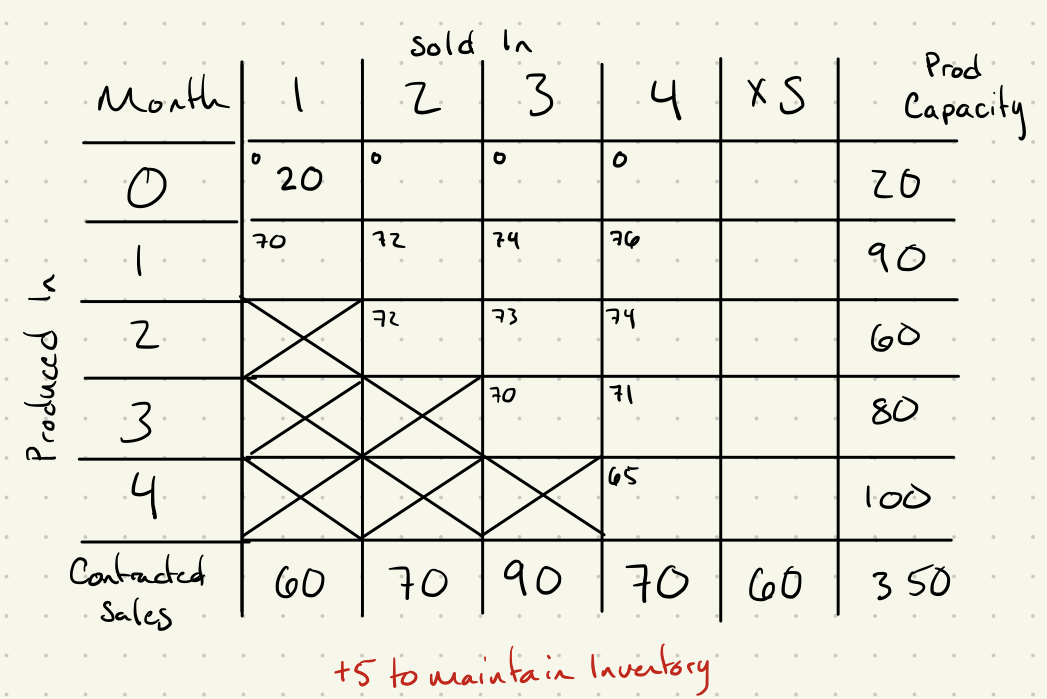
\includegraphics[width=.5\linewidth]{TransportGraph} \\
	The system of linear equations representing this situation 
	will be presented below and will use the following variables: \\
	$z:$ Production costs, \\
	$x_{ps}:$ Products produced in month $p$ and sold in month $s$, \\
	$x_0:$ Is the initial inventory, \\
	$s_p:$ Slack in production capacity for month $p$. \\
	
	\textbf{Linear System Formulated: }
	\begin{flalign*}
		&\text{Min } z = 70x_{11} + 72x_{12} + 74x_{13} + 76x_{14} +72x_{22} + 73x_{23} + 74x_{24} + 70x_{33} + 71x_{34} + 65x_{44}  & \\
		&\text{s.t.}  & 
	\end{flalign*} \vspace{-3em} % x_{} 
	\begin{flalign*}
		\intertext{\small Contracted Sales + GSO Inventory Constraints:}
		x_0 + x_{11} \hspace{18ex} &\geq 65 & \\
		x_0 + x_{12} + x_{22} \hspace{12ex} &\geq 75 & \\
		x_0 + x_{13} + x_{23} + x_{33} \hspace{6ex} &\geq 95 & \\
		x_0 + x_{14} + x_{24} + x_{34} + x_{44} &\geq 75 & \\
		\intertext{\small Production Capacity Constraints:}
		x_0 + s_0 &= 20 & \\
		x_{11} + x_{12} + x_{13} + x_{14} + s_1 &= 90 & \\
		x_{22} + x_{23} + x_{24} + s_2 &= 60 & \\
		x_{33} + x_{34} + s_3 &= 80 & \\
		x_{44} + s_4 &= 100 & 
		\intertext{\small Physics Constraints:}
		x_{11}, x_{12}, x_{13}, x_{14}, x_{22}, x_{23}, x_{24},x_{33}, x_{34}, x_{44}, s_1, s_2, s_3, s_4 &\geq 0 \\
		x_{21}, x_{31}, x_{32}, x_{41}, x_{42}, x_{43} &= 0
	\end{flalign*}
	
	\clearpage
	\part % Q1-C
	\begin{align*} % \xRightarrow[below]{above}
		&\begin{bmatrix}
			2 & 3 & 4 & 3 \\
			4 & 5 & 1 & 2 \\
			1 & 1.5 & 2 & 3/2 \\
		\end{bmatrix}
		\xRightarrow[R1=R1/2]{R3=R3-2R1}
		\begin{bmatrix}
			1 & 1.5 & 2 & 1.5 \\
			4 & 5 & 1 & 2 \\
			0 & 0 & 0 & 0 \\
		\end{bmatrix} 
		\xRightarrow[R1=R1+1.5R2]{R2=R2-4R1} \\
		&\begin{bmatrix}
			1 & 0 & -8.5 & -4.5 \\
			0 & -1 & -7 & -4 \\
			0 & 0 & 0 & 0 \\
		\end{bmatrix}
	\xRightarrow[]{R2=-R2}
	\begin{bmatrix}
		1 & 0 & -8.5 & -4.5 \\
		0 & 1 & 7 & 4 \\
		0 & 0 & 0 & 0 \\
	\end{bmatrix}
	\end{align*}
	
	\textbf{Summary: } The rank of the provided system of equations is 2. As a result, $x_3$ is a free-variable, and there are infinitely many solutions.
	
	\part % Q1-D
	Contribution to $z$: $x_1 = 10/2, x_2=3/1, x_3=12/5$ \\
	Since $x_1$ is the largest, we will maximize it.
	
	\textbf{Summary: } The optimal arrangement will be 
	$x_1=10, x_2=0, x_3=0$ for a maximum $z=100$.
	
\end{parts}
\end{solution}
%\end{ Question 1}

\clearpage

%%%%%%%%%%%%%%%%%%%%%%%%%%%
% 	\begin{ Question 2}	  %
%%%%%%%%%%%%%%%%%%%%%%%%%%%
\question
\begin{parts}
	\part Show that for a $\geq$ constraint $i$ in a maximization problem 
	that $y_i = −(\bar{c}_{BV} B^{−1}\bar{a}_{n+i} )$ 
	
	\part State the dual of the following linear program.
	\begin{flalign*}
		\text{Min } z=3x_1 +7x_2 −15x_3 +43x_4 & & \\
		\text{s.t.} \hspace{2.5em} 
		10x_1 +6x_2 +4x_3 +13x_4 &\leq 100 & \\
		−2x_1 + 3x_2 −5x_3 \hspace{7ex}\, &\geq 200 & \\
		12x_1 −3x_2 +2x_3 +22x_4 &\geq 225 & \\
		x_1,x_3,x_4 \geq 0 x_2 \text{urs} & & \\ 
	\end{flalign*}
	
	\part Given the following final tableau for a maximization problem with all less than or equal to constraints, state the original model. \\
	\begin{tabular}{lllllllll}
		$z$ & $x_1$ & $x_2$ & $x_3$ & $x_4$ & $x_5$ & RHS & BV    & Ratio \\ \hline
		1   & 0     & 0     & 0     & 3/2   & 1     & 36  & Z     &       \\
		0   & 0     & 0     & 1     & 1/3   & -1/3  & 2   & $x_3$ &       \\
		0   & 0     & 1     & 0     & 1/2   & 0     & 6   & $x_2$ &       \\
		0   & 1     & 0     & 0     & -1/3  & 1/3   & 2   & $x_1$ &      
	\end{tabular}

\end{parts}

\clearpage
\begin{solution}
	\begin{parts}
		\part % Q2-A
		As shown by Wayne Winston in his textbook, Operations Research - Applications and Algorithms, we may see that where $BV$ represents the optimal basis for a primal system,
		then \(\bar{c}_{BV} B^{−1}\) is the optimal for both the primal and the dual.
		Furthermore, \(\bar{c}_{BV} B^{−1} = [y_1,y_2,\ldots,y_m]\).
		From this it can be shown that
		\[y_i = \bar{c}_{BV} B^{−1}\bar{a}_{n+i}.\]
		In particular, because the constraint is $\geq$ the coefficients in the corresponding
		column will be negative. Thus,
		\[y_i = -(\bar{c}_{BV} B^{−1}\bar{a}_{n+i}).\]
		
		\part % Q2-B
		\textbf{Summary: } The dual of the provided system is:
		\begin{flalign*}
			\text{Max } z = -100y_1 +200y_2 +225y_3 & & \\
			\text{s.t. }\hspace{2.5em}
			-10y_1 -\quad\, 2y_2 +\ 12y_3 &\leq 3 & \\
			-6y_1 +\quad\ 3y_2 -\ \ 3y_3 &\leq 7 & \\
			-4y_1 -\quad\ 5y_2 +\ \ 2y_3 &\leq -15 & \\
			-13y_1 +\quad \qquad + \ 22y_3 &\leq 43 &
		\end{flalign*}
		
		\part % Q2-C
		\noindent \\
		Exit $x_1$, Re-add $x_5$ \\
		R3 x 3 \\
		R1 + 1/3R3 \\
		R0 - R3 \\
		\begin{tabular}{lllllllll}
			$z$ & $x_1$ & $x_2$ & $x_3$ & $x_4$ & $x_5$ & RHS & BV    & Ratio \\ \hline
			1   & -3    & 0     & 0     & 5/2   & 0     & 30  & Z     &       \\
			0   & 1     & 0     & 1     & 0     & 0     & 4   & $x_3$ &       \\
			0   & 0     & 1     & 0     & 1/2   & 0     & 6   & $x_2$ &       \\
			0   & 3     & 0     & 0     & -1    & 1     & 6   & $x_5$ &      
		\end{tabular} \\
		Exit $x_2$, through $x_4$ \\
		R2 x 2 \\
		R3 + R2 \\
		R0 - 5/2R2 \\
		\begin{tabular}{lllllllll}
			$z$ & $x_1$ & $x_2$ & $x_3$ & $x_4$ & $x_5$ & RHS & BV    & Ratio \\ \hline
			1   & -3    & -5    & 0     & 0     & 0     & 0   & Z     &       \\
			0   & 1     & 0     & 1     & 0     & 0     & 4   & $x_3$ &       \\
			0   & 0     & 2     & 0     & 1     & 0     & 12  & $x_4$ &       \\
			0   & 3     & 2     & 0     & 0     & 1     & 18  & $x_5$ &      
		\end{tabular} \bigskip \\
		\textbf{Summary: } The original model was such that the least common multiple of the coefficients would have have appeared as follows:
		\begin{flalign*}
			\text{Max } z = 3x_1 + 5x_2 & & \\
			\text{s.t.}\hspace{3em}
			x_1 \hspace{6ex} \, &\leq 4 & \\
			2x_2 & \leq 12 & \\
			3x_1 + 2x_2 & \leq 18 & \\
		\end{flalign*}
	\end{parts}
\end{solution}
%\end{ Question 2}

\clearpage

%%%%%%%%%%%%%%%%%%%%%%%%%%%
% 	\begin{ Question 3}	  %
%%%%%%%%%%%%%%%%%%%%%%%%%%%
\question
Jean-Pierre Leveque has recently been named the Minister of International Trade for the new nation of New France. In connection with this position, he has decided that the welfare of the country (and his performance) could best be served by maximizing the net dollar value of the country’s exports for the coming year. (The net dollar value of exports is defined as exports less the cost of all materials imported by the country.) \\ 

The area that now constitutes New France has traditionally made three products for export: steel, heavy machinery, and trucks. For the coming year, Jean-Pierre feels that they could sell all that they could produce of these three items at existing world market prices of \$900/unit for steel, \$2500/unit for machinery, and \$3000/unit for trucks. \\

In order to produce one unit of steel with the country’s existing technology, it takes 0.05 units of machinery, 0.08 units of trucks, two units of ore purchased on the world market for \$100/unit, and other imported materials costing \$100. In addition, it takes .5 man-years of labor to produce each unit of steel. The steel mills of New France have a maximum usable capacity of 300,000 units/year. \\

To produce one unit of machinery requires .75 units of steel, 0.12 units of trucks, and 5 man-years of labor. In addition, \$150 of materials must be imported for each unit of machinery produced. The practical capacity of the country’s machinery plants is 50,000 units/year. \\

In order to produce one unit of trucks, it takes one unit of steel, 0.10 units of machinery, three man-years of labor, and \$500 worth of imported materials. Existing truck capacity is 550,000 units/year. The total manpower available for production of steel, machinery, and trucks is 1,200,000 men/year. \\

To help Jean-Pierre in his planning, he had one of his staff formulate the following model \\

New France Steel Model \\
\begin{flalign*}
	x_1 &= \text{steel production for export} & \hspace{5em} \\
	x_2 &= \text{machine production for export} & \\
	x_3 &= \text{truck production for export} & \\
	x_4 &= \text{total steel production} & \\
	x_5 &= \text{total machine production} & \\
	x_6 &= \text{total truck production} & \\
\end{flalign*}
\begin{align*}
	\text{Max } z = 900x_1 + 2500x_2 + 3000x_3 - 300x_4 -\; 150x_5 - 500x_6 & &&  \\
	\text{s.t.} \hspace{2.7em} 
	- 1x_1 \hspace{21ex}+ 1x_4 - 0.75x_5 -\hspace{2.5ex} 1x_6 &= 0 && \text{Steel Output}  \\
	-x_2 \hspace{9ex} - 0.05x_4\quad + 1x_5 - \  0.1x_6 &= 0 && \text{Machinery Output }  \\
	-x_3 - 0.08x_4 - 0.12x_5 +\quad\! 1x_6 &= 0 && \text{Truck Output}  \\
	x_4 \hspace{17ex} &\leq 300,000 && \text{Steel Capacity}  \\
	x_5 \hspace{8ex} &\leq 50,000 && \text{Machinery Capacity}  \\
	x_6 &\leq 550,000 && \text{Truck Capacity}  \\
	0.5x_4 + 5x_5 + 3x_6 &\leq 1,200,000 && \text{Manpower Avial}  \\ 
	x_1,x_2,x_3,x_4,x_5,x_6 &\geq 0 &&  \\
\end{align*}	
\includegraphics[width=0.9\linewidth]{"Screen Shot 2022-11-14 at 8.31.13 PM"}\\
\includegraphics[width=0.9\linewidth]{"Screen Shot 2022-11-14 at 8.31.30 PM"}\\
\begin{parts}
	\part % Q3-A 
	What would happen to the value of net exports if the world market price of steel increased to \$1225/unit and the country chose to export one unit of steel?
	
	\part % Q3-B
	If New France wants to identify other products it can profitably produce and export, what characteristics should those products have?
	
	\part % Q3-C
	There is a chance that Jean-Pierre may have \$500,000 to spend on expanding capacity. If this investment will buy 500 units of truck capacity, 1000 units of machine capacity, or 300 units of steel capacity, what would be the single best investment?
	
	\part % Q3-D
	If the world market price of the imported materials needed to produce one unit of trucks were to increase by \$400, what would be the optimal export mix for New France, and what would be the dollar value of their net exports?
	
	\part % Q3-E
	The Minister of Defense has recently come to Jean-Pierre and said that he would like to stockpile (inventory) an additional 10,000 units of steel during the coming year. How will this change the constraint equation STEEL, and what impact will it have on net dollar exports?
	
	\part % Q3-F
	A government R\&D group has recently come to Jean-Pierre with a new product, Product X, that can be produced for export with 1.5 man-years of labor and 0.3 units of machinery for each unit produced. What must Product X sell for on the world market to make it attractive for production?
	
	\part % Q3-G
	What is the optimal production and export mix for New France, based the proposed model? What would be the net dollar value of exports under this plan?
	
\end{parts}

\begin{solution}
	\begin{parts}
		\part % Q3-A
		As the New France is utilizing all available steel currently, 
		exporting 1 unit of steel will require reduction in export of another product,
		trucks have the lowest per steel value of secondary product. 
		At a market price of \$1225, exporting one unit of steel will reduce
		revenue by \$1275.
		
		\part % Q3-B
		As there is no steel, but surplus truck capacity and manpower, 
		a change in design or production technique in the truck sector that
		requires more manpower but less of the other supplies would provide
		an opportunity for increase in profit. 
		Reducing the size of vehicles produced for export may have potential, 
		provided the market will consume the new product.
		
		\part % Q3-C
		1585x300 = 475500
		302.5x1000 = 302500
		
		\textbf{Summary: }The increased capacity of 300 units of steel provides the largest net gain under the current method of production. It is probable that this will allow steel to become the new surplus resource instead of truck capacity.
		
		\part % Q3-D
		0.4906250E+09 - (400)262500
		
		\textbf{Summary: }The \$400 dollar decrease is narrowly within the allowable range of decrease on truck profit for this basis to remain optimal. As a result, production should remain the same, but the net export value will be reduced to approximately \$385,625,009.00.
		
		\part % Q3-E
		Machine: 2500 /0.75 = 3333.33 \\
		Truck: 3000 /1 = 3000 \\
		3000\$/truck x 1truck/steel x 10000steel = \$30,000,000 reduced \\
		10000truck x 0.1machine/truck x2500\$/machine = \$2,500,000 added 
		
		\textbf{Summary: }Steel output will need to have a balance of 10,000. 
		Since, under the current system steel is not being exported it will have to be withheld from other industries. Because machines have a higher per export price than trucks,
		it will be better to reduce production of trucks and export the resulting excess machine units. Stockpiling 10,000 units of steel will have a net effect of reducing export revenue by \$27,500,000.
		
		\part % Q3-F
		2500*0.3 = 750 \\
		
		\textbf{Summary: }If the new product sells for more than \$750 it will be more profitable to manufacture and sell it rather than exporting the machine units used to produce it. Additionally, this product can take advantage of the surplus manpower. If sold at \$750 the only gain is diversification of production.
		
		\part % Q3-G
		The recommended production and export mix on the basis of the model provided by Mr. Leveque's staff member is the following: \bigskip\\
		\begin{tabular}{r|l}
			  steel for export & 0 \\
			machine for export & 8750 \\
			  truck for export & 232500 \\
			       total steel production & 300000 \\
			     total machine production & 50000 \\
			       total truck production & 262500 \\
		\end{tabular} \bigskip\\
		For a total revenue of approximately \$490,625,000.
	\end{parts}
\end{solution}
%\end{ Question 3}

\clearpage

%%%%%%%%%%%%%%%%%%%%%%%%%%%
% 	\begin{ Question 4}	  %
%%%%%%%%%%%%%%%%%%%%%%%%%%%
\question
\begin{parts}
	\part Solve the following linear program:
	\begin{flalign*}
		\text{Min } z=4x_1 +5x_2 & & \\
		\text{s.t.} \hspace{2.5em} 
		3x_1 +1x_2 &\leq 27 & \\
		5x_1 +5x_2 &= 60 & \\
		6x_1 +4x_2 &\geq 60 & \\
		x1,x2 &\geq0 & 
	\end{flalign*}

	\part Consider the problem,
	\begin{flalign*}
		\text{Max } z =5x_1 +2x_2 +3x_3 & & \\
		\text{s.t.} \hspace{3em} 
		x_1 +5x_2 +2x_3 &\leq b_1 & \\
		x_1 −5x_2 −6x_3 &\leq b_2 & \\
		x_1,x_2,x_3 &\geq 0 & 
	\end{flalign*}
	where \(b_1\) and \(b_2\) are constants. For specific values of \(b1\) and \(b_2\), the optimal tableau is \\
	\begin{tabular}{ccccccc}
		$z$ & $x_1$ & $x_2$ & $x_3$ & $s_1$ & $s_2$ & RHS \\ \hline
		1   & 0     & $a$   & 7     & $d$   & $e$   & 150 \\
		0   & 1     & $b$   & 2     & 1     & 0     & 30  \\
		0   & 0     & $c$   & -8    & -1    & 1     & 10 
	\end{tabular} \\
	where \(a\), \(b\), \(c\), \(d\), and \(e\) are constants. Determine:
	\begin{subparts}
		\subpart The values of \(b_1\) and \(b_2\) that yield the given optimal solution.
		\subpart The values of \(a\), \(b\), and \(c\) in the optimal tableau.
	\end{subparts}
\end{parts}

\begin{solution}
	\begin{parts}
		\part % Q4-A
		\noindent \\
		\begin{tabular}{cccccccc}
			$z$ & $x_1$ & $x_2$ & $s_1$ & $s_2$ & $A_1$ & RHS & BV    \\ \hline
			1   & -4    & -5    & 0     & 0     & 0     & 0   & -z    \\
			0   & 3     & 1     & 1     & 0     & 0     & 27  & $s_1$ \\
			0   & 5     & 5     & 0     & 0     & 1     & 60  & $A_1$ \\
			0   & -6    & -4    & 0     & 1     & 0     & -60 & $s_2$
		\end{tabular}
		Leaving $A_1$, enter $x_1$ \\
		R3/5 \\
		R1 + 4R3 \\
		R2 - 3R3 \\
		R4 + 6R3 \\
		\begin{tabular}{cccccccc}
			$z$ & $x_1$ & $x_2$ & $s_1$ & $s_2$ & $A_1$ & RHS & BV    \\ \hline
			1   & 0     & -1    & 0     & 0     & 4/5   & 48  & -z    \\
			0   & 0     & -2    & 1     & 0     & -3/5  & -9  & $s_1$ \\
			0   & 1     & 1     & 0     & 0     & 1/5   & 12  & $x_1$ \\
			0   & 0     & 2     & 0     & 1     & 6/5   & 12  & $s_2$
		\end{tabular} \\
		Leaving $s_1$, enter $x_2$ \\
		R2/-2 \\
		R1 + R2 \\
		R3 - R2 \\
		R4 - 2R2 \\
		\begin{tabular}{cccccccc}
			$z$ & $x_1$ & $x_2$ & $s_1$ & $s_2$ & $A_1$ & RHS  & BV    \\ \hline
			1   & 0     & 0     & -1/2  & 0     & 11/10 & 52.5 & -z    \\
			0   & 0     & 1     & -1/2  & 0     & 3/10  & 4.5  & $x_2$ \\
			0   & 1     & 0     & 1/2   & 0     & -1/10 & 7.5  & $x_1$ \\
			0   & 0     & 0     & 1     & 1     & 6/10  & 3    & $s_2$
		\end{tabular} \bigskip \\
		\textbf{Summary: } The optimal situation is $x_1=7.5$ and $x_2=4.5$ for a minimum $z=52.5$.
		
		\part % Q4-B
		\begin{subparts}
			\subpart % Q4-B-1
			The known values in R2 match the values in the original constraints,
			and since $x_1$ has no coefficient, $b_1=30$. 
			Simple substitution into the second constraint or by adding the slack in R3
			gives $b_2=40$.
			\subpart % Q4-B-2
			As above, the values of R2 are unchanged, so $b=5$. 
			Then, undoing the changes to the other rows reveals the remaining numbers.
			For R3, subtracting R2 from the original constraint gives the final R3 and $c=-10$.
			For R1, adding 5R2 to the original function matches the knowns and gives $a=23$.
		\end{subparts}
	\end{parts}
\end{solution}
%\end{ Question 4}

\clearpage

%%%%%%%%%%%%%%%%%%%%%%%%%%%
% 	\begin{ Question 5}	  %
%%%%%%%%%%%%%%%%%%%%%%%%%%%
\question
\begin{parts}
	\part % 5-A
	Consider the following model:
	\begin{flalign*}
		\text{Max} z=3x_1 +1x_2 +2x_3 & & \\
		\text{s.t.} \hspace{2.5em}
		1x_1 −1x_2 +2x_3 &\leq20 & \\
		2x_1 +1x_2 −3x_3 &\leq10 & \\
		x_1,x_2,x_3 &\geq 0 & \\
	\end{flalign*}
	The Final tableau for this problem is: \\
	\begin{tabular}{cccccccc}
		$z$ & $x_1$ & $x_2$ & $x_3$ & $x_4$ & $x_5$ & RHS & BV    \\ \hline
		1   & 8     & 0     & 0     & 3     & 4     & 100 & $z$   \\
		0   & 3     & 0     & 1     & 1     & 1     & 30  & $x_3$ \\
		0   & 5     & 1     & 0     & 1     & 2     & 40  & $x_2$
	\end{tabular} \bigskip \\
	Consider each question below separately; i.e. without regard to the previous question.
	\begin{subparts}
		\subpart % 5-A-i
		Give the range for 1) $b_1$ and 2) $b_2$ over which each could individually range, all other items constant, and maintain the same optimal basis.
		\subpart % 5-A-ii
		If the profit on $c_2$ increased to 5, would the current basis remain optimal?
		\subpart % 5-A-iii
		The organization for which the above model was solved is considering adding a new product, $x_N$. This product uses 2 units of resource 1 and 5 units of resource 2. It’s contribution to profits is \$20 per unit. Should this product be produced? If it is produced, how much should be made?
	\end{subparts}
	\part % 5-B 
	Solve the following goal programming model via the \textbf{simplex method} for goal programs.
	Clearly identify the solution and the level of goal achievement.
	\begin{flalign*}
		\text{Min } z = P_1p_3 + P_2n_4 + P_2p_4 \hspace{20ex}& & \\
		\text{s.t.} \hspace{2.5em} 
		10x_1 +20x_2 +n_1 \hspace{22ex} & =1000 & \\
		20x_1 +10x_2 \hspace{4ex} +n_2 \hspace{18ex} &=800 & \\ 
		5x_1 +10x_2 \hspace{9ex} + n_3 - p_3 \hspace{8ex} &=600 & \\ 
		x_2 \hspace{17ex} + n_4 - p_4 &= 30 &\\
		x_1,x_2,n_1,n_2, n_3,p_3,n_4,p_4 &\geq 0 &
	\end{flalign*}
\end{parts}

\begin{solution}
	\begin{parts}
		\part % 5-A
		\begin{subparts}
			\subpart % 5-A-i
			\begin{multicols}{2}
				\begin{align*}
					b_1 = 20 \\
					\operatorname{max}(\frac{-30}{1},\frac{-40}{1})\leq\Delta&b_1\leq\operatorname{min}() \\
					-30\leq\Delta&b_1 \\
					-10\leq&b_1
				\end{align*}
				\vfill\null
				\begin{align*}
					b_2 = 10 \\
					\operatorname{max}(\frac{-30}{1},\frac{-40}{2})\leq\Delta&b_2\leq\operatorname{min}() \\
					-20\leq\Delta&b_2 \\
					-10\leq&b_2
				\end{align*}
			\end{multicols}
			\textbf{Summary: } As long as both $b$ values remain above $-10$ the provided basis of optimal variables remains the same. Although this may seem counter intuitive at first, this is made possible by second and third coefficients in the constraints being negative.
			
			\subpart % 5-A-ii
			\begin{flalign*}
				c_2 = 1 \\
				\operatorname{max}(\frac{-1}{3},\frac{-2}{4})\leq\Delta&c_2\leq\operatorname{min}() & \\
				-\frac{1}{2}\leq\Delta&c_2 & \\
				\frac{1}{2}\leq&c_2 &
			\end{flalign*}
			\textbf{Summary: } As long as profit associate with $c_2$ remains above $1/2$ this basis is optimal, this is because $x_2$ is not the limiting value within the constraints above that objective coefficient. Any increase only further increases the value of the optimum, which maximizes $x_2$ currently as it is.
			
			\subpart % 5-A-iii
			\(B^{-1}\bar{a}_n = \begin{bmatrix} 7 \\ 12 \end{bmatrix}\) \\
			\(\sum a_iy_i \quad -c_n = 2(3) 5(4) - 20\) \\
			New column \(=\begin{bmatrix} 6 \\ 7 \\ 12 \end{bmatrix}\) \\
			An updated Tableau will be feasible, but because \(\sum a_iy_i \quad -c_n \geq 0\) it may not be optimal. \\
			
			\begin{tabular}{ccccccccc}
				$z$ & $x_1$ & $x_2$ & $x_3$ & $x_4$ & $x_5$ & $x_n$ & RHS & BV    \\ \hline
				1   & -3    & -1    & -2    & 0     & 0     & -20   & 0   & $z$   \\
				0   & 1     & -1    & 2     & 1     & 0     & 2     & 20  & $x_4$ \\
				0   & 2     & 1     & -3    & 0     & 1     & 5     & 10  & $x_5$
			\end{tabular} \\
			\begin{tabular}{ccccccccc}
				$z$ & $x_1$ & $x_2$ & $x_3$ & $x_4$ & $x_5$ & $x_n$ & RHS & BV    \\ \hline
				1   & 5     & 3     & -14   & 0     & 4     & 0     & 40  & $z$   \\
				0   & 1/5   & -16/5 & 11/5  & 1     & -2/5  & 0     & 16  & $x_4$ \\
				0   & 2/5   & 11/5  & -3/5  & 0     & 1/5   & 1     & 2   & $x_n$
			\end{tabular} \\
			\begin{tabular}{ccccccccc}
				$z$ & $x_1$   & $x_2$ & $x_3$ & $x_4$ & $x_5$ & $x_n$ & RHS & BV    \\ \hline
				1   & 33/8    & 17    & 0     & 0     & 23/4  & 0     & 110 & $z$   \\
				0   & 1/16    & -1    & 1     & 5/16  & -2/16 & 0     & 5   & $x_3$ \\
				0   & 511/240 & 8/15  & 0     & 0     & 1/120 & 1     & 5   & $x_n$
			\end{tabular} \\
			
			\textbf{Summary: } The new optimal is $x_3=5, x_n=5$ for an expected profit $z=110$.
			
		\end{subparts}
		\part % 5-B
		\noindent \\
		\begin{tabular}{cccccccccc}
			& $x_1$ & $x_2$ & $n_1$ & $n_2$ & $n_3$ & $n_4$ & $p_3$ & $p_4$ & RHS          \\ \hline
			$P_1$ & 5     & 10    &       &       & 1     &       &       &       & $z_1=600P_1$ \\
			$P_2$ &       & 1     &       &       &       &       &       &       & $z_2=30P_2$  \\ \hline
			& 10    & 20    & 1     &       &       &       &       &       & 1000         \\
			& 20    & 10    &       & 1     &       &       &       &       & 800          \\
			& 5     & 10    &       &       & 1     & -1    &       &       & 600          \\
			&       & 1     &       &       &       &       & 1     & -1    & 30          
		\end{tabular}
		
		\begin{tabular}{cccccccccc}
			& $x_1$ & $x_2$ & $n_1$ & $n_2$ & $n_3$ & $n_4$ & $p_3$ & $p_4$ & RHS          \\ \hline
			$P_1$ &       &       & -1/2  &       & 1     &       &       &       & $z_1=100P_1$ \\
			$P_2$ &       & 1     &       &       &       &       &       &       & $z_2=30P_2$  \\ \hline
			& 1/2   & 1     & 1/20  &       &       &       &       &       & 50           \\
			& 15    &       & -1/2  & 1     &       &       &       &       & 300          \\
			&       &       & -1/2  &       & 1     & -1    &       &       & 100          \\
			&       & 1     &       &       &       &       & 1     & -1    & 30          
		\end{tabular}
		
		\begin{tabular}{cccccccccc}
			& $x_1$ & $x_2$ & $n_1$ & $n_2$ & $n_3$ & $n_4$ & $p_3$ & $p_4$ & RHS         \\ \hline
			$P_1$ &       &       &       &       &       & 1     &       &       & $z_1=0$     \\
			$P_2$ &       & 1     &       &       &       &       &       &       & $z_2=30P_2$ \\ \hline
			& 1/2   & 1     & 1/20  &       &       &       &       &       & 50          \\
			& 15    &       & -1/2  & 1     &       &       &       &       & 300         \\
			&       &       & -1/2  &       & 1     & -1    &       &       & 100         \\
			&       & 1     &       &       &       &       & 1     & -1    & 30         
		\end{tabular}
		
		\begin{tabular}{cccccccccc}
			& $x_1$ & $x_2$ & $n_1$ & $n_2$ & $n_3$ & $n_4$ & $p_3$ & $p_4$ & RHS     \\ \hline
			$P_1$ &       &       &       &       &       & 1     &       &       & $z_1=0$ \\
			$P_2$ &       &       &       &       &       &       & -1    & 1     & $z_2=0$ \\ \hline
			& 1/2   &       & 1/20  &       &       &       & -1    & 1     & 20      \\
			& 15    &       & -1/2  & 1     &       &       &       &       & 300     \\
			&       &       & -1/2  &       & 1     & -1    &       &       & 100     \\
			&       & 1     &       &       &       &       & 1     & -1    & 30     
		\end{tabular}
		
		\begin{tabular}{cccccccccc}
			& $x_1$ & $x_2$ & $n_1$ & $n_2$ & $n_3$ & $n_4$ & $p_3$ & $p_4$ & RHS     \\ \hline
			$P_1$ &       &       &       &       &       & 1     &       &       & $z_1=0$ \\
			$P_2$ &       &       &       &       &       &       & -1    & 1     & $z_2=0$ \\ \hline
			&       &       & 1/30  & -1/30 &       &       & -1    & 1     & 10      \\
			& 1     &       & -1/30 & 1/15  &       &       &       &       & 20      \\
			&       &       & -1/2  &       & 1     & -1    &       &       & 100     \\
			&       & 1     &       &       &       &       & 1     & -1    & 30     
		\end{tabular}
	
		\textbf{Summary: } The goals can be met with $x_2=30$ and $x_1$ is between $20$ and $25$.
	\end{parts}
\end{solution}
%\end{ Question 5}

\end{questions}
\end{document}